\documentclass[twoside]{article}
\usepackage[a4paper]{geometry}
\geometry{verbose,tmargin=2.5cm,bmargin=2cm,lmargin=2cm,rmargin=2cm}
\usepackage{fancyhdr}
\pagestyle{fancy}

% nastavení pisma a~češtiny
\usepackage{lmodern}
\usepackage[T1]{fontenc}
\usepackage[utf8]{inputenc}
\usepackage[czech]{babel}

% odkazy
\usepackage{url}

\usepackage{float}
% vícesloupcové tabulky
\usepackage{multirow}
\usepackage{listings}
\usepackage{xcolor}
\usepackage{amssymb}
\usepackage{gensymb}
\usepackage{bbold}
\usepackage{amsmath}
\usepackage{siunitx}
\usepackage{mathtools}
\usepackage{commath}

% vnořené popisky obrázků
\usepackage{subcaption}

% automatická konverze EPS 
\usepackage{graphicx} 
\usepackage{epstopdf}
\epstopdfsetup{update}

\graphicspath{{./images}}

% odkazy a~záložky
\usepackage[unicode=true, bookmarks=true,bookmarksnumbered=true,
bookmarksopen=false, breaklinks=false,pdfborder={0 0 0},
pdfpagemode=UseNone,backref=false,colorlinks=true] {hyperref}


% Poznámky při překladu
\usepackage{xkeyval}	% Inline todonotes
\usepackage[textsize = footnotesize]{todonotes}
\presetkeys{todonotes}{inline}{}

%https://tex.stackexchange.com/questions/2783/bold-calligraphic-typeface
\DeclareMathAlphabet\mathbfcal{OMS}{cmsy}{b}{n}

% enumerate zacina s pismenem
\renewcommand{\theenumi}{\alph{enumi}}

% smaz aktualni page layout
\fancyhf{}
% zahlavi
\usepackage{titling}
\fancyhf[HC]{\thetitle}
\fancyhf[HLE,HRO]{\theauthor}
\fancyhf[HRE,HLO]{\today}
 %zapati
\fancyhf[FLE,FRO]{\thepage}

% údaje o autorovi
\title{OTE Domácí úkol 7b - Převodník RMS}
\author{Vojtěch Michal}
\date{\today}

%customize code listing
\definecolor{codegreen}{rgb}{0,0.6,0}
\definecolor{codegray}{rgb}{0.5,0.5,0.5}
\definecolor{codepurple}{rgb}{0.58,0,0.82}
\definecolor{backcolour}{rgb}{0.95,0.95,0.92}

\lstdefinestyle{mystyle}{
    backgroundcolor=\color{backcolour},   
    commentstyle=\color{codegreen},
    keywordstyle=\color{magenta},
    numberstyle=\tiny\color{codegray},
    stringstyle=\color{codepurple},
    basicstyle=\ttfamily\footnotesize,
    breakatwhitespace=false,         
    breaklines=true,                 
    captionpos=b,                    
    keepspaces=true,                 
    numbers=left,                    
    numbersep=5pt,                  
    showspaces=false,                
    showstringspaces=false,
    showtabs=false,                  
    tabsize=2
}

\lstset{style=mystyle}

\begin{document}

\maketitle

V simulacích pro tuto úlohu byly použité ideální operační zesilovače bez vstupního napěťového offsetu
a s nulovými vstupními proudy.

\section{Statická převodní charakteristika}

\begin{figure}[h!]
    \centering
    \includegraphics[width=0.55\linewidth]{prevod_char_schema.png}
    \caption{Schéma převodníku efektivní hodnoty}
    \label{fig:prevod_char_schema}
\end{figure}

Pomocí funkce \text{DC sweep} a zapojení na obrázku \ref{fig:prevod_char_schema} byla vykreslena převodní charakteristika na obrázku \ref{fig:prevod_char}.
Stejnosměrné napětí je -- již z definice -- svou vlastní efektivní hodnotou (až na znaménko). Tedy lze očekávat, že převodník RMS se pro DC bude chovat jako obvod absolutní hodnoty.
Kurzory jsou vyznačeny dva body pro vstupní napětí přibližně 0 a 5 V.
V obou dvou je odchylka výstupního napětí od vstupního v řádu desetin milivoltu.


\begin{figure}[h!]
    \centering
    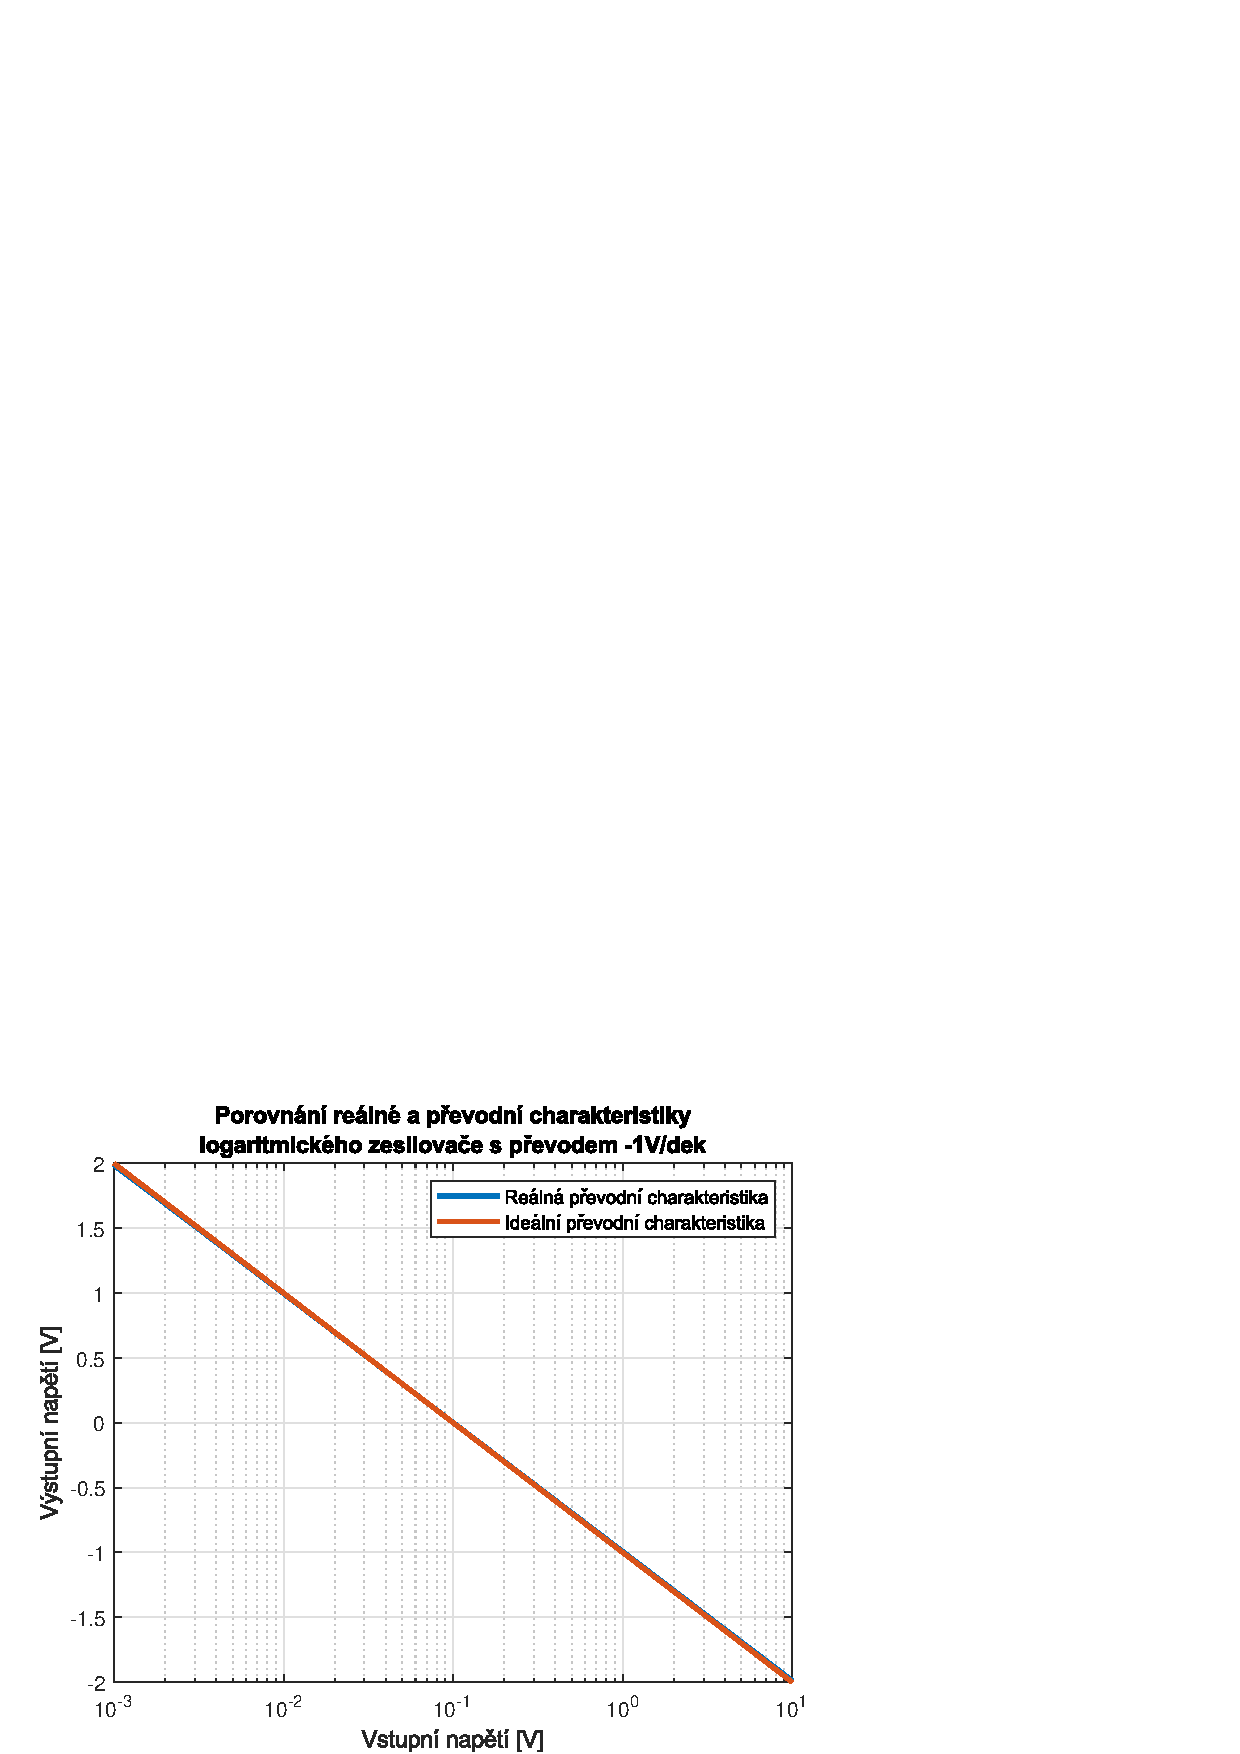
\includegraphics[width=0.55\linewidth]{prevod_char.pdf}
    \caption{Převodní charakteristika obvodu}
    \label{fig:prevod_char}
\end{figure}

\section{Frekvenční charakteristika}

\begin{figure}[h!]
    \centering
    \includegraphics[width=0.8\linewidth]{frek_char_schema.png}
    \caption{Schéma pro získání frekvenční charakteristiky převodníku}
    \label{fig:schema_frek_char}
\end{figure}

Na obrázku \ref{fig:schema_frek_char} je zapojení použité pro získání frekvenční charakteristiky převodníku RMS.
Naměřené hodnoty s použitím vstupního napětí s amplitudou 10 V a proměnnou frekvencí 
jsou uvedené v tabulce \ref{tab:frek_char}.

\begin{table}
    \centering\begin{tabular}{c|c|c}
        vstupní frekvence $f$ & výstupní napětí [V] & zesílení [dB] \\\hline
        1 Hz & 7,058 V & \\
        10 Hz & 7,061 V & \\
        100 Hz & 7,069 V & \\
        1 kHz & 7,067 V & \\
        10 kHz & 7,074 V & \\
        100 kHz & 7,036 V & \\
        500 kHz & 7,005 V & \\
    \end{tabular}
    \caption{Naměřené body frekvenční charakteristiky převodníku RMS}
    \label{tab:frek_char}
\end{table}



\section{Měření efektivní hodnoty různých časových průběhů}

Všechny vstupní signály byly generovány na frekvenci 1 kHz a s maximem $U_m = 10 \si{\volt}$.
Změřená data jsou v tabulce \ref{tab:prubehy}. U obdélníkového signálu byly vyzkoušeny dvě
varianty - signál vystředěný kolem nuly (tedy s rozkmitem $\pm U_m$)
a signál asymetrický (se dvěma hodnotami 0 a $U_m$).

\begin{table}[h]
    \centering
    \begin{tabular}{c|c|c|c}
        tvar signálu & vztah pro efektivní hodnotu & vypočtená RMS & změřená RMS \\ \hline
        harmonický & $\frac{U_m}{\sqrt{2}}$ & 7.07106 \si{\volt} & 7,071 \si{\volt} \\
        trojúhelníkový & $\frac{U_m}{\sqrt{3}}$ & 5.7735 \si{\volt} & 5,943 \si{\volt} \\
        obdélníkový (střída 50 \%, střední hodnota 0) & $U_m$ & 10 \si{\volt} & 10 \si{\volt} \\
        asymetrický obdélníkový (střída 10 \%) & $U_m \sqrt{0,1}$ & 3,162 \si{\volt} & 3,167 \si{\volt} \\
        asymetrický obdélníkový (střída 30 \%) & $U_m \sqrt{0,3}$ & 5,477 \si{\volt} & 5,479 \si{\volt} \\
        asymetrický obdélníkový (střída 50 \%) & $U_m \sqrt{0,5}$ & 7,071 \si{\volt} & 7,072 \si{\volt} \\
        asymetrický obdélníkový (střída 70 \%) & $U_m \sqrt{0,7}$ & 8,367 \si{\volt} & 8,368 \si{\volt} \\
        asymetrický obdélníkový (střída 90 \%) & $U_m \sqrt{0,9}$ & 9,486 \si{\volt} & 9,488 \si{\volt} 
    \end{tabular}
    \caption{Data naměřená pro různé tvary vstupního signálu}
    \label{tab:prubehy}
\end{table}

\end{document}

